% 星屑灯の論文（日本語版）のひな形。山かっこの欄 は tools/stardust_fw/render_report.py が results.json から埋める。
% LuaLaTeX:  lualatex stardust_ja.tex（2 回）
\documentclass[a4paper,twocolumn,10pt]{ltjsarticle}
\usepackage{luatexja}
\usepackage{amsmath,amssymb}
\usepackage{graphicx}
\usepackage{booktabs}
\usepackage[hidelinks]{hyperref}
\usepackage[margin=18mm,columnsep=7mm]{geometry}
\usepackage{caption}
\captionsetup{font=small,labelsep=quad}
\renewcommand{\figurename}{図}
\renewcommand{\tablename}{表}
\newcommand{\us}{\,\mu\mathrm{s}}
\newcommand{\permin}{\,\mathrm{min}^{-1}}
\newcommand{\Iunit}{\,\mathrm{m^{-2}\,s^{-1}\,sr^{-1}}}

\begin{document}

\twocolumn[{%
\begin{center}
{\LARGE\bfseries 卓上ガイガー＝ミュラー管コインシデンス灯\\[2pt]「星屑灯」による宇宙線ミューオンの計測\par}
\vspace{4pt}
{\large\itshape Measuring cosmic-ray muons with a desktop Geiger--Müller coincidence lamp\par}
\vspace{8pt}
{\large MONORADIO\par}
\vspace{2pt}
{\small 2026 年 11 月　·　\url{https://github.com/monoradio102/stardust-lamp}\par}
\end{center}
\vspace{4pt}
\begin{quote}\small
\textbf{要旨}　上下に重ねた 2 本のガイガー＝ミュラー（GM）管が同時に反応したときだけ光るランプ「星屑灯」を，宇宙線ミューオンの計数器として評価した．屋内の机上で 10.0 時間の連続観測を行い，1,162 事象の同時計数を得た．計数率は $R = 1.94 \pm 0.06\permin$ である．1 分ごとの計数はポアソン分布に（$\chi^2$ 検定 $p = 0.1$），到来間隔は指数分布に（KS 検定 $p = 0.4$）従い，到来が独立な事象の列であることを確かめた．偶然同時計数は理論式 $R_\mathrm{acc} = 2\tau R_A R_B$ どおりで，全体の 0.04\% にとどまる．管の寸法と天頂角分布 $I(\theta) = I_0\cos^2\theta$ から幾何学的因子をモンテカルロ法で求め，鉛直強度 $I_0 = 51.3$--$72.5\Iunit$ を得た．これは文献値（約 70）と整合する．ファームウェアの異なる 45.7 時間の観測（同じ放電の二重計数を補正）とも，計数率は誤差の範囲で一致した．

\smallskip
\textbf{キーワード}　宇宙線，ミューオン，GM 計数管，同時計数法，ポアソン過程，幾何学的因子
\end{quote}
\vspace{6pt}
}]

\section{はじめに}

一次宇宙線は，主に銀河内の超新星残骸で加速された陽子や原子核である．これが上空 15\,km 前後で大気の原子核と衝突し，$\pi$ 中間子を経てミューオンが生まれる．地上に届く荷電粒子の大部分はこのミューオンであり，水平な面 1\,cm$^2$ あたり毎分およそ 1 個が通過する\cite{pdg}．

ミューオンを数える古典的な方法は，2 つ以上の検出器を重ね，すべてが同時に反応した事象だけを選ぶ同時計数法である．単独の GM 管は環境のガンマ線にも反応するが，2 本を同時に貫く粒子は，地上ではほぼミューオンに限られる．

星屑灯は，この同時計数をアナログ回路で行い，その結果を LED の光として見せる照明である（図~\ref{fig:lamp}）．本研究の目的は，この装置が定量的な測定器として使えることを示すことにある．具体的には，(i)~到来の統計の検証，(ii)~偶然同時計数の理論式の検証，(iii)~管の幾何からの計数率の予言と鉛直強度の推定，(iv)~2 回の観測による再現性の確認，を報告する．

\begin{figure}[t]
\centering
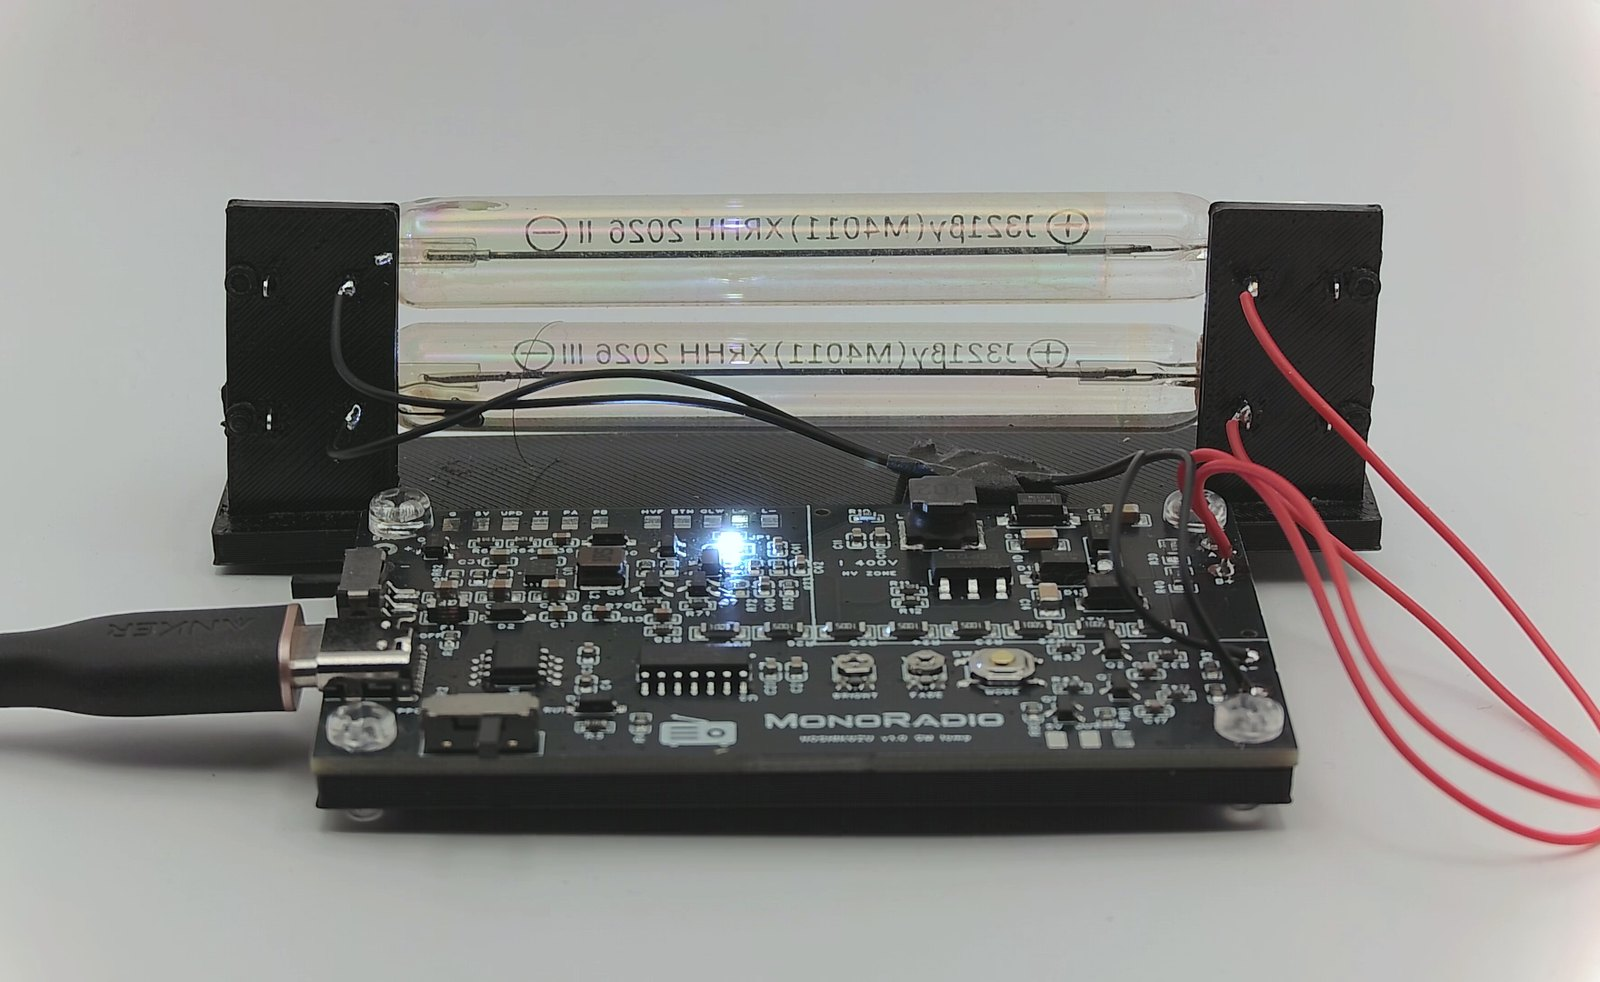
\includegraphics[width=\columnwidth]{../../../hardware/images/lamp.jpg}
\caption{星屑灯．上下に重ねた 2 本の GM 管（奥）と，同時計数の瞬間に光る基板（手前）．}
\label{fig:lamp}
\end{figure}

\section{装置と方法}

\subsection{検出器}

検出器は GM 管 J321 を 2 本，軸を水平にして上下に重ねたものである（表~\ref{tab:setup}，図~\ref{fig:detector}）．高圧はブースト回路と倍電圧回路で作り，マイコンが帰還をかけて 360\,V に保つ．

\begin{table}[t]
\centering\small
\caption{検出器と観測の条件}
\label{tab:setup}
\begin{tabular}{@{}ll@{}}
\toprule
GM 管 & J321 × 2（外径 10\,mm，ガラス長 70\,mm）\\
配置 & 軸を水平に上下に重ねる．中心間隔 約 12\,mm \\
印加電圧 & 360\,V（観測 B の実測 359.2--360.1\,V）\\
同時の窓 & $\tau = 100\us$ \\
不感時間 & $\tau_d = 200\us$（管ごと，1.5.0 以降）\\
場所 & 屋内，机の上 \\
\bottomrule
\end{tabular}
\end{table}

\begin{figure*}[t]
\centering
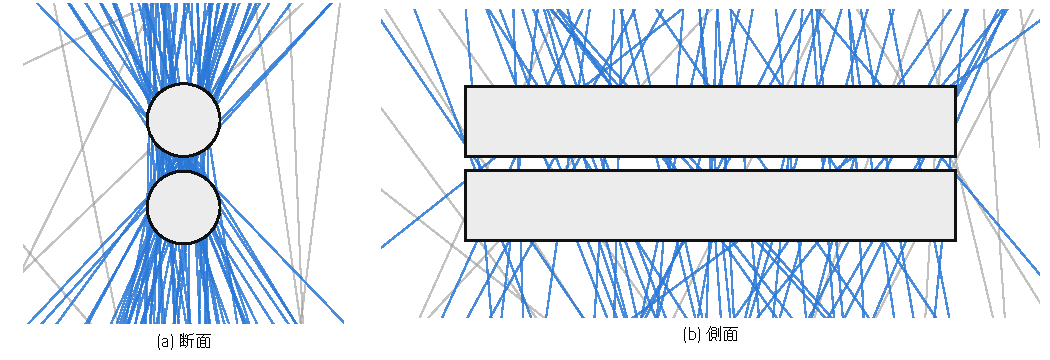
\includegraphics[width=\textwidth]{figures/ja/detector.pdf}
\caption{検出器の幾何．モンテカルロで発生させた直線のうち，2 本の管を両方とも通るもの（青，計数される）と，そうでないもの（灰）．}
\label{fig:detector}
\end{figure*}

\subsection{同時計数と計数系}

同時計数は 2 段で行う．光は，2 本の管のパルスが重なっている間だけ，2 段の PNP トランジスタを通してコンデンサに電荷が入ることで生じる．窓はパルスの重なりで決まり，約 0.1\,ms である．計数は，マイコン（ATtiny1614）が各管のパルスの立ち下がりを割り込みで捉え，時刻を $\mu$s 単位で記録して行う．2 本の時間差が $|\Delta t| \le \tau$ のとき同時計数とする．あわせて，窓を 1\,ms ずらした遅延同時計数 $D$ を数える．同じ管のパルスが，直前に数えたパルスから $\tau_d = 200\us$ 以内に来た場合は，同じ放電の再パルスとみなして数えない（不感時間，ファームウェア 1.5.0 以降）．非まひ型の不感時間による数え落としは，真の計数率を $n$，観測した計数率を $m$ として $n = m/(1 - m\tau_d)$ で補正できる\cite{knoll}．単独の管で 20\,min$^{-1}$ でも $m\tau_d \approx 7\times10^{-5}$ であり，補正は無視できる．本論文の数値はすべてデジタルの計数による．

\subsection{データ取得}

基板を USB で小型 PC に接続し，(1)~10 秒ごとの集計（高圧，管 A・B の計数，同時計数 $C$，遅延同時計数 $D$），(2)~反応 1 回ごとの事象と PC 側の時刻（ms），(3)~$|\Delta t| \le 5$\,ms の組について基板側で測った $\Delta t = t_B - t_A$（$\mu$s）を記録した．観測は 2 回行った（表~\ref{tab:runs}）．主な結果は観測 B による．観測 A は第~\ref{sec:compare} 節で，再現性の確認に用いる．どちらの観測でも，10 秒ごとの記録に 25 秒を超える欠落はなかった．

\begin{table}[t]
\centering\small
\caption{観測}
\label{tab:runs}
\begin{tabular}{@{}lccr@{}}
\toprule
 & FW & 開始（JST） & 時間 \\
\midrule
観測 A & 1.4.0 & 2026-11-07 11:01 & 45.7\,h \\
観測 B & 1.6.0 & 2026-11-09 09:30 & 10.0\,h \\
\bottomrule
\end{tabular}
\end{table}

\section{結果}

\subsection{計数率}

観測 B の計数を表~\ref{tab:rates} に示す．単独の計数は，大部分が環境のガンマ線による．

\begin{table}[t]
\centering\small
\caption{計数と計数率（観測 B）}
\label{tab:rates}
\begin{tabular}{@{}lrr@{}}
\toprule
 & 計数 & 計数率 [min$^{-1}$] \\
\midrule
同時計数 $C$ & 1,162 & $1.937 \pm 0.057$ \\
管 A & 10,302 & 17.17 \\
管 B & 8,130 & 13.55 \\
遅延同時計数 $D$ & 1 & --- \\
\bottomrule
\end{tabular}
\end{table}

\subsection{到来の統計}
\label{sec:stat}

到来が互いに独立で，計数率 $R$ が一定なら，時間 $\Delta T$ の計数 $k$ はポアソン分布に従い，到来間隔 $\Delta t$ は指数分布に従う．
\begin{gather}
P(k) = \frac{\lambda^{k} e^{-\lambda}}{k!}, \qquad \lambda = R\,\Delta T, \label{eq:poisson}\\
p(\Delta t) = R\, e^{-R\Delta t}, \qquad \Delta t_{1/2} = \frac{\ln 2}{R}. \label{eq:expo}
\end{gather}
1 分ごとの計数の平均は 1.93，分散は 1.765 で，ポアソン分布の性質 $\sigma^2 = \lambda$ に合う（図~\ref{fig:poisson}）．分布全体の $\chi^2$ 検定は $\chi^2 = 9.2$（自由度 5，$p = 0.1$）であった．到来間隔の中央値は 22.3\,s で，式~\eqref{eq:expo} の $\Delta t_{1/2} = 21.5$\,s と一致する（図~\ref{fig:intervals}）．指数分布との KS 検定は $p = 0.4$ であった．どちらの検定でも，独立な到来という仮説は棄却されない．

\begin{figure}[t]
\centering
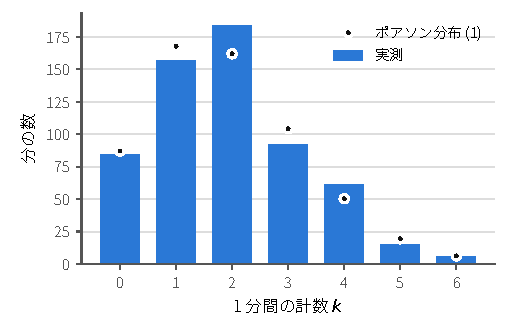
\includegraphics[width=\columnwidth]{figures/ja/poisson.pdf}
\caption{1 分ごとの同時計数の分布（599 分）．点は式~\eqref{eq:poisson}（$\lambda = 1.93$）．}
\label{fig:poisson}
\end{figure}

\begin{figure}[t]
\centering
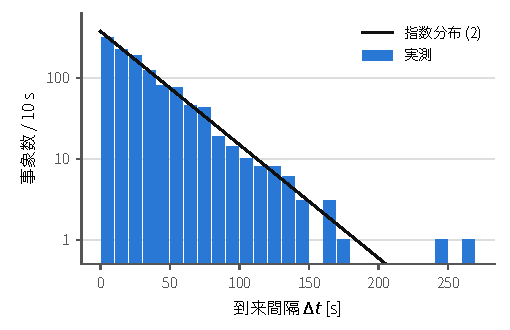
\includegraphics[width=\columnwidth]{figures/ja/intervals.pdf}
\caption{同時計数の到来間隔の分布（1,161 個）．線は式~\eqref{eq:expo}．}
\label{fig:intervals}
\end{figure}

\subsection{偶然同時計数}

互いに無関係な 2 本の反応が，たまたま窓に入る率は
\begin{equation}
R_\mathrm{acc} = 2\,\tau\, R_A\, R_B \label{eq:acc}
\end{equation}
である．観測 B では，窓の中の偶然同時計数の期待値は 0.47 事象で，同時計数全体の 0.04\% にあたる．窓の外（$0.1 < |\Delta t| \le 5$\,ms）の組はすべて偶然の重なりなので，時間差の分布は平らになり，その高さは式~\eqref{eq:acc} で決まる（図~\ref{fig:coinc}）．窓の外の組は実測 17 組，予測 22.8 組であった．遅延同時計数 $D$ も，予測 0.94 事象に対して実測 1 事象であった．

\begin{figure}[t]
\centering
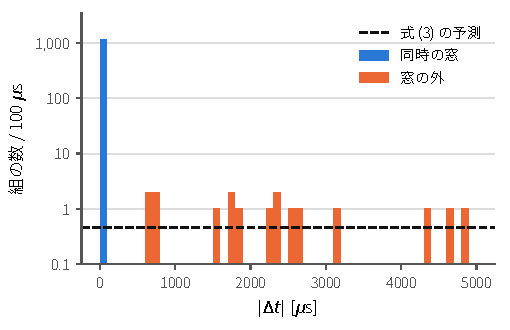
\includegraphics[width=\columnwidth]{figures/ja/coincidence.pdf}
\caption{2 本の管の時間差 $|\Delta t|$ の分布（100\,$\mu$s ごと）．破線は式~\eqref{eq:acc} から求めた偶然同時計数の高さ．}
\label{fig:coinc}
\end{figure}

\subsection{時間差分布}

ミューオンは約 12\,mm 離れた 2 本の管を 0.04\,ns で通り抜ける．一方，測った時間差の中央値は $+16\us$ で，同時計数の 89\% が $+9$--$+17\us$ に集まる（図~\ref{fig:dt}）．この差は粒子の飛行時間ではなく，マイコンが 2 本の割り込みを順に処理する時間による．2 本の管の信号は同じポートの割り込みで受け，マイコンは管 A から順に処理する．そのため $\Delta t$ は管 A の処理時間だけ正にずれる（平均 $+15.8\us$）．管 B がわずかに早く立ち下がると処理の順が入れ替わり，$-21.4\us$ 付近に小さな山（全体の 9.5\%）ができる．

\begin{figure}[t]
\centering
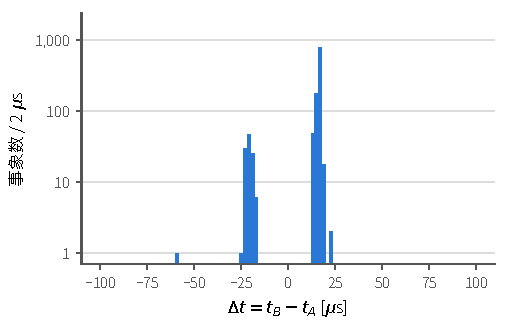
\includegraphics[width=\columnwidth]{figures/ja/dt.pdf}
\caption{窓の中の時間差 $\Delta t = t_B - t_A$ の分布．}
\label{fig:dt}
\end{figure}

\subsection{時間的な安定性}

観測 B の 1 時間ごとの計数は平均 116.6 で，ばらつきの $\chi^2$ は 6.3（自由度 8，$p = 0.62$）であった．観測 A（補正後）も $\chi^2 = 49.9$（自由度 43，$p = 0.22$）で，統計的な揺れを超える変化は見られない（図~\ref{fig:hourly}）．

\begin{figure*}[t]
\centering
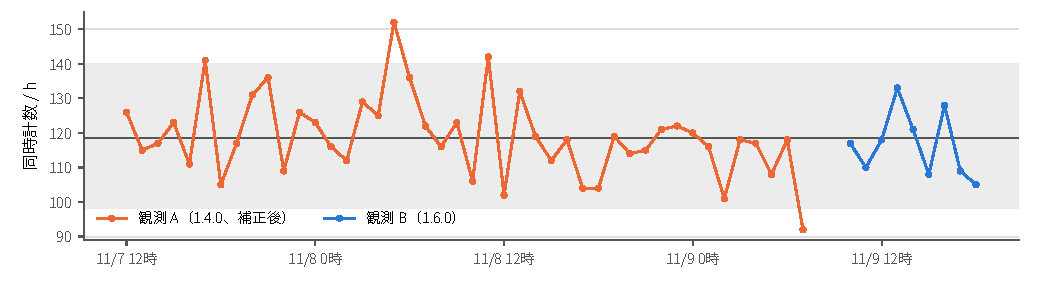
\includegraphics[width=\textwidth]{figures/ja/hourly.pdf}
\caption{1 時間ごとの同時計数．帯はポアソン分布で 95\% が入る範囲，線は平均．観測 A は第~\ref{sec:compare} 節の補正を施した値．}
\label{fig:hourly}
\end{figure*}

\subsection{2 回の観測の比較}
\label{sec:compare}

観測 A は，不感時間を入れる前のファームウェア（1.4.0）で行った．その事象列には，10\,ms 以内に同時計数が 2--4 回続く塊が 1 時間あたり 6.8 回あった．到来が独立なら，45 時間でおよそ 2 回しか起きない並びである．塊の中では，片方の管が最初のパルスから 20--96\,$\mu$s 遅れて再びパルスを出し，それが窓に入って同じミューオンを重ねて数えていた．時間差を 5\,ms まで広げても，100\,$\mu$s より外に再パルスの過剰はなかった．

補正前の計数率は 2.14\,min$^{-1}$ で，1 時間ごとのばらつきもポアソン分布より大きかった（$\chi^2 = 62.5$，自由度 43，$p = 0.027$）．PC 側の時刻で 10\,ms 以内に続いた反応を 1 回の放電にまとめると，$\chi^2 = 49.9$（$p = 0.22$）でポアソンの揺れに収まり，計数率は $1.98 \pm 0.03\permin$ となった．不感時間を入れた観測 B の $1.94 \pm 0.06\permin$ とは，差が 0.7\,$\sigma$ で一致する（表~\ref{tab:compare}）．観測 B では塊は 1 時間あたり 0.0 回，同じ管の 10\,ms 以内の再反応は 5.1 回で，偶然に重なる期待値 4.8 回と変わらない．平均値だけでは気づきにくい誤りも，事象ごとの時刻を残しておけば，第~\ref{sec:stat} 節と同じ統計の検定で見つけて補正できる．

\begin{table}[t]
\centering\small
\caption{2 回の観測の比較．$\chi^2$ は 1 時間ごとの計数のばらつき，塊は 10\,ms 以内に続く同時計数．}
\label{tab:compare}
\setlength{\tabcolsep}{4pt}
\begin{tabular}{@{}lccc@{}}
\toprule
 & \multicolumn{2}{c}{観測 A} & 観測 B \\
 & 補正前 & 補正後 & \\
\midrule
計数率 [min$^{-1}$] & 2.14 & $1.98 \pm 0.03$ & $1.94 \pm 0.06$ \\
$\chi^2$/自由度 & 62.5/43 & 49.9/43 & 6.3/8 \\
その $p$ 値 & 0.027 & 0.22 & 0.62 \\
塊 [h$^{-1}$] & 6.8 & --- & 0.0 \\
\bottomrule
\end{tabular}
\end{table}

\section{幾何学的受け入れと鉛直強度}

地上のミューオンの強度は，天頂角 $\theta$ に対して近似的に
\begin{equation}
I(\theta) = I_0 \cos^2\theta \label{eq:cos2}
\end{equation}
と表される\cite{pdg}．方向 $(\theta,\phi)$ について，2 本の管を両方とも通る直線の束をその方向に垂直な面へ射影した面積を $A_\perp(\theta,\phi)$ とすると，計数率は
\begin{equation}
R = \varepsilon\, I_0\, G, \qquad G \equiv \int_\Omega \cos^2\theta\, A_\perp(\theta,\phi)\, d\Omega \label{eq:G}
\end{equation}
となる．$\varepsilon$ は検出効率と遮へいを含む係数である．幾何学的因子 $G$ は，水平面を通る直線を $\cos^3\theta$ の重みで発生させるモンテカルロ法で求めた．GM 管の有感長は直接測れないので，ガラス長 7\,cm と，両端の電極部を除いた 5\,cm の 2 通りで計算した（表~\ref{tab:geo}）．

\begin{table}[t]
\centering\small
\caption{幾何学的因子と計数率の予測（$I_0 = 70\Iunit$，$\varepsilon = 1$）}
\label{tab:geo}
\begin{tabular}{@{}ccccc@{}}
\toprule
有感長 & $G$ [cm$^2$\,sr] & 予測 & 実測 & 実測/予測 \\
\midrule
5\,cm & 4.45 & 1.87 & 1.94 & 1.04 \\
7\,cm & 6.29 & 2.64 & 1.94 & 0.73 \\
\bottomrule
\end{tabular}
\end{table}

$\varepsilon = 1$ として式~\eqref{eq:G} を逆に解くと，$I_0 = R/G = 51.3$--$72.5\Iunit$ となる．この範囲は文献値の約 $70\Iunit$\cite{pdg} を含む．屋内の遮へいと検出効率による $\varepsilon < 1$ を考えると，整合的である．計数されるミューオンの天頂角の中央値は 27° である（図~\ref{fig:zenith}）．強度は鉛直方向で最大だが，天頂付近の立体角が小さいため，分布の山は 20--30° に来る．計数率の予測と鉛直強度の系統誤差としては，有感長の不確かさ（表~\ref{tab:geo} の幅），検出効率と屋内の遮へい（$\varepsilon$），中心間隔の測定誤差（1\,mm で $G$ が約 8\% 変わる）がある．

\begin{figure}[t]
\centering
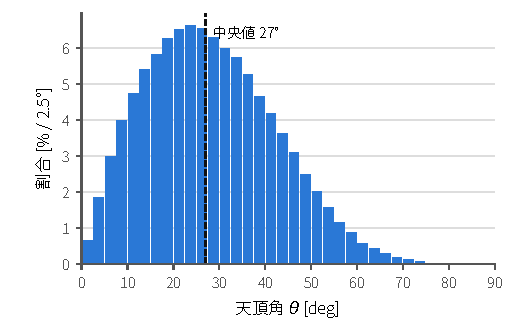
\includegraphics[width=\columnwidth]{figures/ja/zenith.pdf}
\caption{計数されるミューオンの天頂角の分布（モンテカルロ，有感長 7\,cm）．}
\label{fig:zenith}
\end{figure}

\section{考察：時間の遅れ}

ミューオンの寿命は $\tau_\mu = 2.197\us$ であり\cite{pdg}，光速で飛んでも $c\tau_\mu \approx 659$\,m しか進めない．それでも上空 15\,km で生まれたミューオンが地上で数えられるのは，特殊相対論の時間の遅れによる\cite{rossi,frisch}．
\begin{equation}
\gamma = \frac{E}{m_\mu c^2}, \quad L = \gamma\beta c\tau_\mu, \quad \frac{N(h)}{N_0} = e^{-h/L} \label{eq:dilation}
\end{equation}
地上での典型的なエネルギー $E \approx 4$\,GeV では $\gamma \approx 38$，$L \approx 25$\,km となり，15\,km 先まで残る割合は 0.55 である．時間の遅れがなければ $1.3\times 10^{-10}$ にすぎない（大気中のエネルギー損失は無視した概算）．毎分約 2 回の同時計数は，時間の遅れが実際に起きていることの，ささやかな証拠でもある．

\section{結論}

装飾用のランプとして作った星屑灯が，宇宙線ミューオンの定量的な計数器として機能することを示した．同時計数率は $1.94 \pm 0.06\permin$ で，到来はポアソン過程に従う．偶然同時計数は式~\eqref{eq:acc} どおりで全体の 0.04\% にとどまる．管の幾何と $\cos^2\theta$ 分布からの予測は実測と整合し，鉛直強度 $I_0 = 51.3$--$72.5\Iunit$ を得た．事象ごとの記録の検定で計数系の二重計数を見つけて補正でき，補正後の 2 回の観測は誤差の範囲で一致した．

\section{今後の研究}

計数の相対統計誤差は $\sigma_R/R = 1/\sqrt{N}$ である．本装置 1 台では 1 日に約 2,789 事象を数え，1 日の計数率を $\pm1.9$\% で決められる．2 本の並びを管の軸のまわりに角度 $\alpha$ だけ傾けると，受け入れる天頂角が変わる．式~\eqref{eq:G} から予測した計数率の比を図~\ref{fig:tilt} に示す．各角度で 1 日ずつ測れば式~\eqref{eq:cos2} を検証できる．このほか，気圧効果（$\Delta R/R = \beta\Delta P$，$\beta \approx -0.1$ から $-0.2$\,\%/hPa\cite{dorman}），太陽活動による減少（フォーブッシュ減少\cite{forbush}），2 台による空気シャワーの検出，場所による違いの測定が可能である．

\begin{figure}[t]
\centering
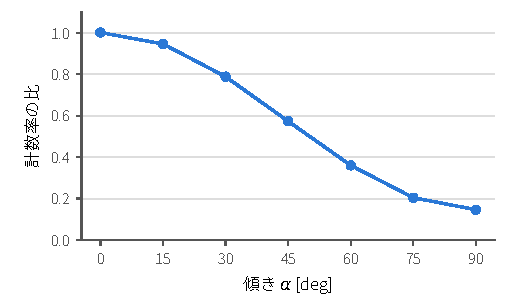
\includegraphics[width=\columnwidth]{figures/ja/tilt.pdf}
\caption{2 本の並びを傾けたときの計数率の比の予測（$\alpha = 0°$ が上下，90° が横並び）．}
\label{fig:tilt}
\end{figure}

\section*{データとコード}

解析コード，結果の数値，データ，回路図，ファームウェアは \url{https://github.com/monoradio102/stardust-lamp} で公開している．

\begin{thebibliography}{9}\small
\bibitem{pdg} S.~Navas \textit{et al.} (Particle Data Group), Phys.\ Rev.\ D \textbf{110}, 030001 (2024).
\bibitem{rossi} B.~Rossi and D.~B.~Hall, Phys.\ Rev.\ \textbf{59}, 223 (1941).
\bibitem{frisch} D.~H.~Frisch and J.~H.~Smith, Am.\ J.\ Phys.\ \textbf{31}, 342 (1963).
\bibitem{knoll} G.~F.~Knoll, \textit{Radiation Detection and Measurement}, 4th ed.\ (Wiley, 2010).
\bibitem{dorman} L.~I.~Dorman, \textit{Cosmic Rays in the Earth's Atmosphere and Underground} (Springer, 2004).
\bibitem{forbush} S.~E.~Forbush, Phys.\ Rev.\ \textbf{51}, 1108 (1937).
\end{thebibliography}

\end{document}
